% (c) 2012-2013 Dimitrios Vrettos - d.vrettos@gmail.com

\chapter{Problemi di primo grado}

\section{Un po' di storia}

Sin dall'antichità l'uomo si è
trovato di fronte a difficoltà pratiche, legate alla vita quotidiana
e ha perciò messo a punto strategie per superarle.

Sembra che nell'antico Egitto le periodiche piene del
Nilo abbiano spinto l'uomo a sviluppare la capacità
di tracciare rette parallele, rette perpendicolari, di misurare il
perimetro e l'area di particolari figure geometriche o
viceversa di calcolare le misure dei lati di poligoni di dato perimetro
o data area per poter ridefinire i confini degli appezzamenti di
terreno.

Il \emph{papiro di Rhind}\footnote{Dal nome dell'inglese A.~H.~Rhind che lo comprò a Luxor nel~1858.}, testo egizio scritto in
ieratico, risalente al~1700~\aC, si autodefinisce
``istruzioni per conoscere tutte le cose
oscure'' e contiene più di~85 problemi con relativi
metodi di soluzione riguardanti il calcolo della capacità di
recipienti e di magazzini, la ricerca dell'area di
appezzamenti di terreno e altre questioni aritmetiche.

Nel problema~24 del papiro, ad esempio, viene calcolato il mucchio
quando esso ed il suo settimo sono uguali a~19. Mucchio è
l'incognita del problema, indicata con il termine
\emph{aha} il cui segno è
% (c) 2012 Dimitrios Vrettos - d.vrettos@gmail.com
\begin{hieroglyph}{\leavevmode \loneSign{{\Hsmaller\Aca GD/66/}}}\end{hieroglyph}.


Noi traduciamo la richiesta nell'equazione~$x+\dfrac{1}{7}x=19$.

Nel~1202 Leonardo Pisano, conosciuto col nome paterno di
``filius Bonacci'' o Fibonacci, pubblicò il
\emph{Liber Abaci} in cui, a partire dall'ottavo
capitolo, presenta vari metodi algebrici per la risoluzione di problemi
di matematica applicata, legati alla realtà
dell'epoca, in particolare
all'ambiente commerciale. I nuovi
``algoritmi'' presentati da Fibonacci,
intendevano facilitare la risoluzione dei problemi di calcolo evitando
l'utilizzo dell'abaco. Nel~1223 a
Pisa, l'imperatore Federico~II di Svevia, assistette a
un singolare torneo tra matematici dell'epoca; il
problema proposto era il seguente:

<<Quante coppie di conigli si ottengono in un anno (salvo i
casi di morte) supponendo che ogni coppia dia alla luce
un'altra coppia ogni mese e che le coppie più
giovani siano in grado di riprodursi già al secondo mese di
vita?>>.

Fibonacci vinse la gara dando al quesito una risposta così rapida da
far persino sospettare che il torneo fosse truccato. La soluzione fu
trovata tramite l'individuazione di una particolare
successione di numeri, nota appunto come successione di Fibonacci.

Secondo la leggenda, il grande matematico Carl Fiedrich Gauss\footnote{matematico, astronomo e fisico tedesco (1777 - 1855).} già
all'età di tre anni avrebbe corretto un errore di
suo padre nel calcolo delle sue finanze. All'età di
10 anni fu autorizzato a seguire le lezioni di aritmetica di un certo
Buttner. Un giorno, agli studenti particolarmente turbolenti, Buttner
diede come compito di punizione il calcolo della somma dei primi~100
numeri naturali, da~1 a~100. Poco dopo, sorprendendo tutti, il giovanissimo Carl
diede la risposta esatta, ``\np{5050}''.
Si era accorto che mettendo in riga tutti i numeri da~1 a~100 e nella
riga sottostante i numeri da~100 a~1, ogni colonna dava come somma~101;
fece dunque il prodotto~$100\times~101$ e divise per~2, ottenendo facilmente il
risultato. Buttner rimase sgomento.

\section{Risoluzione dei problemi}

 \epigraph{La risoluzione dei problemi [\ldots] serve ad acuire
 l'ingegno e a dargli la facoltà di penetrare
 l'intera ragione di tutte le cose.}{{\scshape{R. Descartes}}}

I problemi che possono presentarsi nel corso degli studi o
nell'attività lavorativa sono di diversa natura: di
tipo economico, scientifico, sociale, possono riguardare insiemi
numerici o figure geometriche. La matematica ci può aiutare a
risolvere i problemi quando essi possono essere tradotti in
``forma matematica'', quando cioè
è possibile trascrivere in simboli le relazioni che intercorrono
tra le grandezze del problema.

Analizzeremo problemi di tipo algebrico o geometrico, che potranno
essere formalizzati attraverso equazioni di primo grado in una sola
incognita. Prima di buttarci alla risoluzione del problema, procediamo
a:

\begin{enumeratea}
\item una lettura ``attenta'' del
testo al fine di individuare l'ambiente del problema,
le parole chiave, i dati e le informazioni implicite,
l'obiettivo;
\item la scelta della grandezza incognita e la descrizione
dell'insieme in cui si ricerca il suo valore,
ragionando sull'obiettivo del problema (condizioni sull'incognita);
\item la traduzione in ``forma matematica'' delle relazioni che intercorrono tra i
dati e l'obiettivo, cioè l'individuazione dell'equazione risolvente;
\item la risoluzione dell'equazione trovata;
\item il confronto tra la soluzione trovata e le condizioni poste su di essa.
\end{enumeratea}

\begin{problema}
 Un mattone pesa un chilo più mezzo mattone. Quanto pesa un mattone?
\end{problema}

\begin{soluzione}
 La situazione può essere materialmente descritta con nella figura~1.
Togliamo da ogni piatto della bilancia mezzo mattone, la bilancia è
ancora in equilibrio come mostra la figura~2, da ciò possiamo
dedurre che mezzo mattone pesa un chilo. Il mattone intero pesa dunque
due chili.
\begin{center}
 % (c) 2012 Dimitrios Vrettos - d.vrettos@gmail.com
\begin{tikzpicture}[font=\small,x=5mm, y=5mm, scale=.75]

\begin{scope}[fill=black, draw=black]
\filldraw (0,0) rectangle (4,1);
\filldraw[rounded corners=2] (1,1.1)rectangle (3,1.6);
\filldraw (1.8,1.7) rectangle (2.3,8);
\filldraw[rounded corners=2] (1.5,8.1)rectangle (2.6,8.6);
\filldraw (-4,8.7) rectangle (8,9.1);
\filldraw[rounded corners=2] (1.8,8.8)rectangle (2.3,9.8);

\node[name=c1,shape=semicircle,shape border rotate=180, inner sep=3.75mm,draw=black, fill=black] at (-4,3)
{};
\node (a) at (-4,8.7) {};
\draw (a.center)--(c1.arc start);
\draw (a.center)--(c1.arc end);

\node[name=c2,shape=semicircle,shape border rotate=180, inner sep=3.75mm,draw=black, fill=black] at (8,3)
{};
\node (b) at (8,8.7) {};
\draw (b.center)--(c2.arc start);
\draw (b.center)--(c2.arc end);

\filldraw[fill=orange, draw=orange](-5.5,4.02) rectangle (-2.5,5.1);
\filldraw[fill=orange, draw=orange](6.5,4.02) rectangle (8,5.1);
\filldraw[fill=white] (8.3,4) rectangle (9.7,5.1);
\filldraw[fill=white] (8.6,5.1) rectangle (9.4,5.4);
\node () at (9,4.5) {1kg};
\node () at (2,-1) {Figura 1};
\end{scope}

\begin{scope}[fill=black, draw=black, xshift=100mm]
\filldraw (0,0) rectangle (4,1);
\filldraw[rounded corners=2] (1,1.1)rectangle (3,1.6);
\filldraw (1.8,1.7) rectangle (2.3,8);
\filldraw[rounded corners=2] (1.5,8.1)rectangle (2.6,8.6);
\filldraw (-4,8.7) rectangle (8,9.1);
\filldraw[rounded corners=2] (1.8,8.8)rectangle (2.3,9.8);

\node[name=c1,shape=semicircle,shape border rotate=180, inner sep=3.75mm,draw=black, fill=black] at (-4,3)
{};
\node (a) at (-4,8.7) {};
\draw (a.center)--(c1.arc start);
\draw (a.center)--(c1.arc end);

\node[name=c2,shape=semicircle,shape border rotate=180, inner sep=3.75mm,draw=black, fill=black] at (8,3)
{};
\node (b) at (8,8.7) {};
\draw (b.center)--(c2.arc start);
\draw (b.center)--(c2.arc end);

\filldraw[fill=orange, draw=orange](-5,4.02) rectangle (-3,5.1);
\filldraw[fill=white] (7.3,4) rectangle (8.7,5.1);
\filldraw[fill=white] (7.6,5.1) rectangle (8.4,5.4);
\node () at (8,4.5) {1kg};
\node () at (2,-1) {Figura 2};
\end{scope}

\end{tikzpicture}
\end{center}

Risolviamo ora il problema seguendo la procedura sopra suggerita:

\emph{Dati}: peso di un mattone~$=$ peso di mezzo mattone~$+ 1\unit{kg}.$

\emph{Obiettivo}: peso del mattone.

\emph{Procedura risolutiva}:

Come incognita del problema possiamo scegliere il peso del mattone: la
indichiamo con~$p$.
Il valore di~$p$ dovrà essere un numero positivo.
L'equazione risolvente è la traduzione con formalismo
matematico dell'unica relazione contenuta nel testo del
problema:~$p=1+\frac{1}{2}p$.

Risolviamo l'equazione:~$p-\frac{1}{2}p=1\:\Rightarrow\:\frac{1}{2}p=1\:\Rightarrow\: p=2\unit{kg}.$
La soluzione ottenuta è accettabile; il problema è determinato.
\end{soluzione}

\begin{problema}
 Aggiungendo ad un numero naturale i suoi tre quarti, si ottiene il suo
doppio aumentato di~10. Qual è il numero?
\end{problema}

\begin{soluzione}
L'ambiente del problema è numerico: si cerca un numero
naturale. Indichiamo con~$n$ l'incognita
cerchiamo quindi~$n\in\insN$. La lettura attenta del testo mette
in luce le operazioni che dobbiamo eseguire
sull'incognita e che traduciamo nei dati:

\emph{Dati}:~$n+\dfrac{3}{4}n=2n+10$.

\emph{Obiettivo}:~$n\in\insN$.

\emph{Procedura risolutiva}:

L'equazione risolvente è già indicata nei dati~$n+\dfrac{3}{4}n=2n+10$.

Per risolverla moltiplichiamo ambo i membri per~4, otteniamo:
\[4n+3n-8n=40\quad\Rightarrow\quad -n=40\quad\Rightarrow\quad n=-40.\]

La soluzione non è accettabile per le condizioni poste; il problema
non ha soluzione.
\end{soluzione}

\begin{problema}
 Il~1{\textdegree} gennaio~1990 Chiara aveva il doppio
dell'età di Aldo; il~1{\textdegree} gennaio~2000
Chiara aveva vent'anni più di Aldo. Qual era
l'età di Chiara il~1{\textdegree} gennaio~2010?
\end{problema}

\begin{soluzione}
Leggendo attentamente il problema notiamo che le incognite sono due:
l'età di Chiara e l'età di Aldo.
Indichiamo perciò con~$c$ l'età di
Chiara al~1990 e con~$a$ quella di Aldo.

Nel~2000 la loro età sarà aumentata di~10 anni. Naturalmente la
soluzione del problema sarà nell'insieme dei numeri
naturali. Scriviamo dati e obiettivo usando il formalismo matematico:

\emph{Dati}: nel~1990:~$c=2a$, nel~2000:~$c+10=(a+10)+20$.

\emph{Obiettivo}: L'età di Chiara nel~2010.

\emph{Procedura risolutiva}:
Osserviamo che una volta determinata l'età di Chiara
nel~1990, basterà aggiungere a questa~20 per ottenere la soluzione,
pertanto l'età di Chiara nel~2010 è~$c+20$.
Trasformiamo la seconda relazione riportata nei dati sostituendo
l'informazione relativa al~1990,
si ottiene~$2a+10=a+10+20\Rightarrow 2a-a=20\Rightarrow a=20$.
L'età di Aldo nel~1990 era~20, quindi~$c=40$.
Dunque, l'età di Chiara nel~2010 era~$c+20=40+20=60$.
La soluzione è accettabile; il problema è determinato.
\end{soluzione}

\begin{problema}
 Calcolare l'area di un rettangolo in cui
l'altezza supera $\dfrac{1}{3}$ della base di~8m e il
perimetro è~$\dfrac{20}{7}$ della base stessa.
\end{problema}

\begin{soluzione}
 Il problema è di tipo geometrico e riguarda un rettangolo. Facendo riferimento alla figura abbiamo:
\begin{multicols}{2}
 \emph{Dati}:~$\overline{AD}=\dfrac{1}{3}\overline{AB}+8$, $\quad 2p=\dfrac{20}{7}\overline{AB}$.

\emph{Obiettivo}: L'$\Area (ABCD).$

\begin{center}
 % (c) 2012 Dimitrios Vrettos - d.vrettos@gmail.com
\begin{tikzpicture}[font=\small,x=8mm, y=3.5mm]

\draw (0,0) rectangle (4,4);

\begin{scope}[left]
\node  at (0,4) {$A$};
\node  at (0,0) {$D$};
\end{scope}

\begin{scope}[right]
\node  at (4,4) {$B$};
\node  at (4,0) {$C$};
\end{scope}
\end{tikzpicture}
\end{center}
\end{multicols}

\emph{Procedura risolutiva}:
$\Area (ABCD)=\text{ misura base }\cdot \text{ misura altezza }=\overline{AB}\cdot \overline{AD}$.

Dobbiamo dunque determinare queste due misure. I dati del problema
indicano che la misura dell'altezza dipende da quella
della base; una volta trovata questa misura basta farne un terzo e
aggiungere~8 per avere quella dell'altezza; questo
ragionamento ci fa scegliere come incognita~$\overline{AB}=x$
con~$x$ numero reale positivo.

Traduciamo con formalismo matematico la prima e la seconda relazione
contenuta nei dati:
$\overline{AD}=\dfrac{1}{3}x+8$ e~$2p=\dfrac{20}{7}x$.

Sappiamo che il perimetro di un rettangolo è il doppio della somma
della base con l'altezza. Riscriviamo con linguaggio
matematico anche questa relazione:~$2\cdot \left(x+\dfrac{1}{3}x+8\right)=\dfrac{20}{7}x$
che risulta l'equazione risolvente.

Svolgiamo i calcoli e otteniamo~$4x=21\cdot 16\Rightarrow x=84\Rightarrow\overline{AB}=84$ e quindi~$\overline{AD}=36$.
Ottenute le misure della base e dell'altezza calcoliamo~$\Area (ABCD)=36\cdot 84=\np[m^2]{3024}$.
\end{soluzione}

\begin{problema}
In un triangolo rettangolo il perimetro è~$120\unit{cm}$ e un cateto è~$3/5$
dell'ipotenusa. Determinare l'area del
triangolo.
\end{problema}

\begin{soluzione}
 Il problema è di tipo geometrico e riguarda un triangolo rettangolo.
Rappresentiamo il triangolo:

\begin{multicols}{2}

\emph{Dati}:~$C\hat{A}B=$ angolo retto, $2p= 120$, $\overline{AC}=\dfrac{3}{5}\overline{CB}$.

\emph{Obiettivo}: L'$\Area (ABC)$.
\begin{center}
 % (c) 2012 Dimitrios Vrettos - d.vrettos@gmail.com
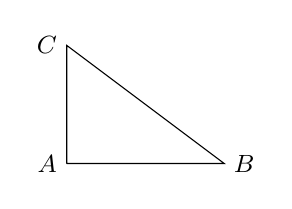
\begin{tikzpicture}[font=\small,x=5mm, y=5mm]

\draw (0,0)-- (4,0)--(0,3)--(0,0);

 \begin{scope}[left]
\node  at (0,3) {$C$};
\node  at (0,0) {$A$};
\end{scope}

\node[right]  at (4,0) {$B$};

\end{tikzpicture}
\end{center}
\end{multicols}



\emph{Procedura risolutiva}:~$\Area (ABC) =\dfrac{1}{2}\overline{AB}\cdot \overline{AC}$.

Per calcolare l'area, occorre determinare la misura dei
cateti del triangolo rettangolo; i dati del problema ci danno una
relazione tra la misura di un cateto e la misura
dell'ipotenusa; conosciamo anche il perimetro del
triangolo.

Scegliamo come incognita la misura in cm di~$\overline{CB}$, cioè
$\overline{CB}=x$ con~$x\in\insR^{+}$.

\emph{Formalizziamo i dati}:
 \begin{equation}\label{16.1}
 \overline{CB} =x;\quad \overline{AC} =\dfrac{3}{5}x;\quad \overline{AB} +x+\dfrac{3}{5}x=120.
 \end{equation}


Per poter scrivere un'equazione che ci permetta di determinare il
valore dell'incognita ci manca la misura di $\overline{AB}$. Sembra
che il problema sia privo di un'informazione. Tuttavia, il triangolo
dato è rettangolo, quindi tra i suoi lati sussiste la relazione del
teorema di Pitagora:
$\overline {CB}^{2}=\overline {AB}^{2}+\overline {AC}^{2}$.

Pertanto possiamo determinare la misura di~$\overline{AB}$:
\[\overline{AB}=\sqrt{\overline{CB}^{2}-\overline {AC}^{2}}=\sqrt{x^{2}-\left(\frac{3}{5}x\right)^{2}}=\sqrt{\frac{16}{25}x^{2}}=\frac{4}{5}x.\]

Con questo dato riscriviamo la \ref{16.1} che risulta essere
l'equazione risolvente del problema
\[\frac{4}{5}x+x+\dfrac{3}{5}x=120\quad\Rightarrow\quad 12x=120\cdot 5\quad\Rightarrow\quad x=50\quad\Rightarrow\quad\overline{CB}=50.\]

Quindi~$\overline {AC} = 30\unit{cm}$ e~$\overline {AB}= 40\unit{cm}\quad\Rightarrow\quad\Area (ABC)=\dfrac{30\cdot 40}{2}=600\unit{cm}^{2}$.
\end{soluzione}

\newpage
% (c) 2012 Claudio Carboncini - claudio.carboncini@gmail.com
% (c) 2012-2014 Dimitrios Vrettos - d.vrettos@gmail.com
\section{Esercizi}
\subsection{Esercizi dei singoli paragrafi}
\subsubsection*{\thechapter.1 - Quadrato di un binomio}
\begin{multicols}{2}
\begin{esercizio}
\label{ese:16.1}
Quando è possibile, scomponi in fattori, riconoscendo il quadrato di un binomio.
\begin{enumeratea}
 \item $a^{2}-2a+1$;
 \item $x^{2}+4x+4$;
 \item $y^{2}-6y+9$;
 \item $16t^{2}+8t+1$;
 \item $4x^{2}+1+4x$;
 \item $9a^{2}-6a+1$.
\end{enumeratea}
\end{esercizio}

\begin{esercizio}
\label{ese:16.2}
Quando è possibile, scomponi in fattori, riconoscendo il quadrato di un binomio.
\begin{enumeratea}
 \item $4x^{2}-12x+9$;
 \item $\dfrac{1}{4}a^{2}+ab+b^{2}$;
 \item $9x^{2}+4+12x$;
 \item $\dfrac{4}{9}a^{{4}}-4a^{2}+9$;
 \item $\dfrac{1}{4}x^{2}-\dfrac{1}{3}x+\dfrac{1}{9}$;
 \item $16a^{2}+\dfrac{1}{4}b^{2}-4ab$.
\end{enumeratea}
\end{esercizio}

\begin{esercizio}
\label{ese:16.3}
Quando è possibile, scomponi in fattori, riconoscendo il quadrato di un binomio.
\begin{enumeratea}
 \item $-9x^{2}-\dfrac{1}{4}+3x$;
 \item $4x^{2}+4xy+y^{2}$;
 \item $a^{4}+36a^{2}+12a^{3}$;
 \item $144x^{2}-6xa^{2}+\dfrac{1}{16}a^{4}$;
 \item $x^{2}-6xy+9y^{2}$;
 \item $-x^{2}-6xy-9y^{2}$.
\end{enumeratea}
\end{esercizio}

\begin{esercizio}
\label{ese:16.4}
Quando è possibile, scomponi in fattori, riconoscendo il quadrato di un binomio.
\begin{enumeratea}
 \item $25+10x+x^{2}$;
 \item $\dfrac{1}{4}x^{2}+\dfrac{1}{3}xy+\dfrac{1}{9}y^{2}$;
 \item $25-10x+x^{2}$;
 \item $\dfrac{9}{25}a^{4}-6a^{2}+25$;
 \item $4x^{2}+2x^{4}+1$;
 \item $4x^{2}-4x^{4}-1$.
\end{enumeratea}
\end{esercizio}

\begin{esercizio}
\label{ese:16.5}
Quando è possibile, scomponi in fattori, riconoscendo il quadrato di un binomio.
\begin{enumeratea}
 \item $-a^{3}-2a^{2}-a$;
 \item $3a^{7}b-6a^{5}b^{2}+3a^{3}b^{3}$;
 \item $100+a^{2}b^{4}+20ab^{2}$;
 \item $2x^{13}-8x^{8}y+8x^{3}y^{2}$;
 \item $x^{8}+8x^{4}y^{2}+16y^{4}$;
 \item $-x^{2}+6{xy}+9y^{2}$.
\end{enumeratea}
\end{esercizio}

\begin{esercizio}
\label{ese:16.6}
Quando è possibile, scomponi in fattori, riconoscendo il quadrato di un binomio.
\begin{enumeratea}
 \item $4a^{2}b^{4}-12ab^{3}+9b^{6}$;
 \item $a^{2}+a+1$;
 \item $36a^{6}b^{3}+27a^{5}b^{4}+12a^{7}b^{2}$;
 \item $25x^{14}+9y^{6}+30x^{7}y^{3}$;
 \item $-a^{7}-25a^{5}+10a^{6}$;
 \item $25a^{2}+49b^{2}+35ab$.
\end{enumeratea}
\end{esercizio}

\begin{esercizio}
\label{ese:16.7}
Quando è possibile, scomponi in fattori, riconoscendo il quadrato di un binomio.
\begin{enumeratea}
 \item $4y^{6}+4-4y^{2}$;
 \item $\dfrac{1}{4}a^{2}+2ab+b^{2}$;
 \item $25a^{2}-10{ax}-x^{2}$;
 \item $9x^{2}+4y^{2}-6{xy}$.
\end{enumeratea}
\end{esercizio}
\end{multicols}

\begin{esercizio}
\label{ese:16.8}
Individua perché i seguenti polinomi non sono quadrati di un binomio.
\begin{enumeratea}
 \item $4x^{2}+4xy-y^{2}$\, non è un quadrato di binomio perché\,\dotfill;
 \item $x^{2}-6xy+9y$\, non è un quadrato di binomio perché\dotfill;
 \item $25+100x+x^{2}$\, non è un quadrato di binomio perché\dotfill;
 \item $\dfrac{1}{4}x^{2}+\dfrac{2}{3}xy+\dfrac{1}{9}$\, non è un quadrato di binomio perché\dotfill;
 \item $25t^{2}+4-10t$\, non è un quadrato di binomio perché\dotfill%ex103
\end{enumeratea}
\end{esercizio}

\begin{multicols}{2}
\begin{esercizio}[\Ast]
\label{ese:16.9}
Quando è possibile, scomponi in fattori, riconoscendo il quadrato di un binomio.
\begin{enumeratea}
 \item $24a^{3}+6a+24a^{2}$;
 \item $3a^{2}x-12axb+12b^{2}x$;
 \item $5a^{2}+2ax+\dfrac{1}{5}x^{2}$;
 \item $x^{6}y+x^{2}y+2x^{4}y$.
\end{enumeratea}
\end{esercizio}

\begin{esercizio}[\Ast]
\label{ese:16.10}
Quando è possibile, scomponi in fattori, riconoscendo il quadrato di un binomio.
\begin{enumeratea}
 \item $x^{5}+4x^{4}+4x^{3}$;
 \item $2y^{3}-12y^{2}x+18x^{2}y$;
 \item $-50t^{3}-8t+40t^{2}$;
 \item $2^{10}x^{2}+2^{6}\cdot 3^{20}+3^{40}$.
\end{enumeratea}
\end{esercizio}

\begin{esercizio}[\Ast]
\label{ese:16.11}
Quando è possibile, scomponi in fattori, riconoscendo il quadrato di un binomio.
\begin{enumeratea}
 \item $2^{20}x^{40}-2^{26}\cdot x^{50}+2^{30}\cdot x^{60}$;
 \item $10^{100}x^{50}-2\cdot 10^{75}x^{25}+10^{50}$.
\end{enumeratea}
\end{esercizio}

\begin{esercizio}[\Ast]
\label{ese:16.12}
Quando è possibile, scomponi in fattori, riconoscendo il quadrato di un binomio.
\begin{enumeratea}
 \item $10^{11}x^{10}-2\cdot 10^{9}x^{5}+10^{6}$;
 \item $x^{2n}+2x^{n}+1$.
\end{enumeratea}
\end{esercizio}
\end{multicols}

\subsubsection*{\thechapter.2 - Quadrato di un polinomio}
\begin{multicols}{2}
\begin{esercizio}
\label{ese:16.13}
Quando è possibile, scomponi in fattori, riconoscendo il quadrato di un polinomio.
\begin{enumeratea}
 \item $a^{2}+b^{2}+c^{2}+2ab+2ac+2bc$;
 \item $x^{2}+y^{2}+z^{2}+2xy-2xz-2yz$;
 \item $x^{2}+y^{2}+4+4x+2xy+4y$;
 \item $4a^{4}-6{ab}-4a^{2}b+12a^{3}+b^{2}+9a^{2}$.
\end{enumeratea}
\end{esercizio}

\begin{esercizio}
Quando è possibile, scomponi in fattori, riconoscendo il quadrato di un polinomio.
\label{ese:16.14}
\begin{enumeratea}
 \item $9x^{6}+2y^{2}z+y^{4}-6x^{3}z-6x^{3}y^{2}+z^{2}$;
 \item $\dfrac{1}{4}a^{2}+b^{4}+c^{6}+ab^{2}+{ac}^{3}+2b^{2}c^{3}$;
 \item $a^{2}+2ab+b^{2}-2a+1-2b$;
 \item $x^{2}+\dfrac{1}{4}y^{2}+4-xy+4x-2y$.
\end{enumeratea}
\end{esercizio}

\begin{esercizio}
\label{ese:16.15}
Quando è possibile, scomponi in fattori, riconoscendo il quadrato di un polinomio.
\begin{enumeratea}
 \item $a^{2}+b^{2}+c^{2}-2ac-2bc+2ab$;
 \item $-x^{2}-2xy-9-y^{2}+6x+6y$;
 \item $4a^{2}+4ab-8a+b^{2}-4b+4$;
 \item $a^{2}b^{2}+2a^{2}b+a^{2}-2ab^{2}-2ab+b^{2}$.
\end{enumeratea}
\end{esercizio}
\end{multicols}
\begin{esercizio}
Individua perché i seguenti polinomi non sono quadrati.
\label{ese:16.16}
\begin{enumeratea}
 \item $a^{2}+b^{2}+c^{2}$\, non è un quadrato perché\dotfill;
 \item $x^{2}+y^{2}+4+4x+4xy+4y$\, non è un quadrato perché\dotfill;
 \item $a^{2}+b^{2}+c^{2}-2ac-2bc-2ab$\, non è un quadrato perché\dotfill;
 \item $a^{2}+b^{2}-1-2a-2b+2ab$\, non è un quadrato perché\dotfill
\end{enumeratea}
\end{esercizio}

\begin{esercizio}[\Ast]
\label{ese:16.17}
Quando è possibile, scomponi in fattori, riconoscendo il quadrato di un polinomio.
\begin{enumeratea}
 \item $a^{2}+4ab-2a+4b^{2}-4b+1$;
 \item $a^{2}b^{2}+2a^{2}b+a^{2}+4ab^{2}+4ab+4b^{2}$;
 \item $x^{2}-6xy+6x+9y^{2}-18y+9$.
\end{enumeratea}
\end{esercizio}

\begin{esercizio}
\label{ese:16.18}
Quando è possibile, scomponi in fattori, riconoscendo il quadrato di un polinomio.
\begin{enumeratea}
 \item $x^{4}+2x^{3}+3x^{2}+2x+1$\quad  scomponi prima \quad~$3x^{2}=x^{2}+2x^{2}$;
 \item $4a^{4}+8a^{2}+1+8a^{3}+4a$\quad  scomponi prima \quad~$8a^{2}=4a^{2}+4a^{2}$;
 \item $9x^{4}+6x^{3}-11x^{2}-4x+4$ \quad scomponi in maniera opportuna \quad~$-11x^{2}$.
\end{enumeratea}
\end{esercizio}

\begin{esercizio}
\label{ese:16.19}
Quando è possibile, scomponi in fattori, riconoscendo il quadrato di un polinomio.
\begin{enumeratea}
 \item $25x^{2}-20ax-30bx+4a^{2}+12ab+9b^{2}$;
 \item $2a^{10}x+4a^{8}x+2a^{6}x+4a^{5}x+4a^{3}x+2x$;
 \item $a^{2}+b^{2}+c^{2}+d^{2}-2ab+2ac-2ad-2bc+2bd-2cd$;
 \item $x^{6}+x^{4}+x^{2}+1+2x^{5}+2x^{4}+2x^{3}+2x^{3}+2x^{2}+2x$.
\end{enumeratea}
\end{esercizio}

\subsubsection*{\thechapter.3 - Cubo di un binomio}
\begin{multicols}{2}
\begin{esercizio}
\label{ese:16.20}
Quando è possibile, scomponi in fattori, riconoscendo il cubo di un binomio.
\begin{enumeratea}
 \item $8a^{3}+b^{3}+12a^{2}b+6ab^{2}$;
 \item $b^{3}+12a^{2}b-6ab^{2}-8a^{3}$;
 \item $-12a^{2}+8a^{3}-b^{3}+6ab$;
 \item $-12a^{2}b+6ab+8a^{3}-b^{3}$.
\end{enumeratea}
\end{esercizio}

\begin{esercizio}
\label{ese:16.21}
Quando è possibile, scomponi in fattori, riconoscendo il cubo di un binomio.
\begin{enumeratea}
 \item $-x^{3}+6x^{2}-12x+8$;
 \item $-x^{9}-3x^{6}+3x^{3}+8$;
 \item $x^{3}y^{6}+1+3x^{2}y^{2}+3xy^{2}$;
 \item $x^{3}+3x-3x^{2}-1$.
\end{enumeratea}
\end{esercizio}

\begin{esercizio}
\label{ese:16.22}
Quando è possibile, scomponi in fattori, riconoscendo il cubo di un binomio.
\begin{enumeratea}
 \item $-5x^{5}y^{3}-5x^{2}-15x^{4}y^{2}-15x^{3}y$;
 \item $-a^{6}+27a^{3}+9a^{5}-27a^{4}$;
 \item $64a^{3}-48a^{2}+12a-1$;
 \item $a^{6}+9a^{4}+27a^{2}+27$.
\end{enumeratea}
\end{esercizio}

\begin{esercizio}
\label{ese:16.23}
Quando è possibile, scomponi in fattori, riconoscendo il cubo di un binomio.
\begin{enumeratea}
 \item $x^{3}-x^{2}+\dfrac{1}{3}x-\dfrac{1}{27}$;
 \item $0,001x^{6}+0,015x^{4}+0,075x^{2}+0,125$;
 \item $\dfrac{27}{8}a^{3}-\dfrac{27}{2}a^{2}x+18ax^{2}-8x^{3}$;
 \item $x^{3}-x^{2}+\dfrac{1}{3}x-\dfrac{1}{27}$.
\end{enumeratea}
\end{esercizio}

\begin{esercizio}
\label{ese:16.24}
Individua perché i seguenti polinomi non sono cubi.
\begin{enumeratea}
 \item $a^{10}-8a-6a^{7}+12a^{4}$\, non è un cubo perché\dotfill;
 \item $27a^{3}-b^{3}+9a^{2}b-9ab^{2}$\, non è un cubo perché\dotfill;
 \item $8x^{3}+b^{3}+6x^{2}b+6{xb}^{2}$\, non è un cubo perché\dotfill;
 \item $x^{3}+6ax^{2}-6a^{2}x+8a^{3}$\, non è un cubo perché\dotfill
\end{enumeratea}
\end{esercizio}

\begin{esercizio}
\label{ese:16.25}
Quando è possibile, scomponi in fattori, riconoscendo il cubo di un binomio.
\begin{enumeratea}
 \item $x^{3}-6x^{2}+12x-8$;
 \item $a^{3}b^{3}+12ab+48ab+64$;
 \item $216x^{3}-540ax^{2}+450a^{2}x-125a^{3}$;
 \item $8x^{3}+12x^{2}+6x+2$.
\end{enumeratea}
\end{esercizio}

\begin{esercizio}[\Ast]
\label{ese:16.26}
Quando è possibile, scomponi in fattori, riconoscendo il cubo di un binomio.
\begin{enumeratea}
 \item $a^{6}+3a^{4}b^{2}+3a^{2}b^{4}+b^{6}$;
 \item $8a^{3}-36a^{2}b+54ab^{2}-27b^{3}$;
 \item $a^{6}+3a^{5}+3a^{4}+a^{3}$;
 \item $a^{10}-8a-6a^{7}+12a^{4}$.%ex154b trovato risultato: a\left(a^3-2\right)^3
\end{enumeratea}
\end{esercizio}

\begin{esercizio}
\label{ese:16.27}
Quando è possibile, scomponi in fattori, riconoscendo il cubo di un binomio.
\begin{enumeratea}
 \item $8x^{3}-36x^{2}+54x-27$;
 \item $x^{6}+12ax^{4}+12a^{2}x^{2}+8a^{3}$;
 \item $x^{300}-10^{15}-3\cdot 10^{5}x^{200}+3\cdot 10^{10}x^{100}$;
 \item $a^{6n}+3a^{4n}x^{n}+3a^{2n}x^{2n}+x^{3n}$.
\end{enumeratea}
\end{esercizio}
\end{multicols}
\begin{esercizio}
\label{ese:16.28}
Quando è possibile, scomponi in fattori, riconoscendo il cubo di un binomio.
\begin{enumeratea}
 \item $10^{15}a^{60}+3\cdot 10^{30}a^{45}+3\cdot 10^{45}a^{30}+10^{60}a^{15}$;
 \item $10^{-33}x^{3}-3\cdot 10^{-22}x^{2}+3\cdot 10^{-11}x-1$.
\end{enumeratea}
\end{esercizio}

\subsubsection*{\thechapter.4 - Differenza di due quadrati}
\begin{multicols}{2}
\begin{esercizio}
\label{ese:16.29}
Scomponi i seguenti polinomi come differenza di quadrati.
\begin{enumeratea}
 \item $a^{2}-25b^{2}$;
 \item $16-x^{2}y^{2}$;
 \item $25-9x^{2}$;
 \item $4a^{4}-9b^{2}$;
 \item $x^{2}-16y^{2}$;
 \item $144x^{2}-9y^{2}$.
\end{enumeratea}
\end{esercizio}

\begin{esercizio}
\label{ese:16.30}
Scomponi i seguenti polinomi come differenza di quadrati.
\begin{enumeratea}
 \item $16x^{4}-81z^{2}$;
 \item $a^{2}b^{4}-c^{2}$;
 \item $4x^{6}-9y^{4}$;
 \item $-36x^{8}+25b^{2}$;
 \item $-1+a^{2}$;
 \item $\dfrac{1}{4}x^{4}-\dfrac{1}{9}y^{4}$.
\end{enumeratea}
\end{esercizio}

\begin{esercizio}
\label{ese:16.31}
Scomponi i seguenti polinomi come differenza di quadrati.
\begin{enumeratea}
 \item $\dfrac{a^{2}}{4}-\dfrac{y^{2}}{9}$;
 \item $2a^{2}-50$;
 \item $a^{3}-16{ab}^{6}$;
 \item $-4x^{2}y^{2}+y^{2}$;
 \item $-4a^{2}+b^{2}$;
 \item $25x^{2}y^{2}-\dfrac{1}{4}z^{6}$.
\end{enumeratea}
\end{esercizio}

\begin{esercizio}
\label{ese:16.32}
Scomponi i seguenti polinomi come differenza di quadrati.
\begin{enumeratea}
 \item $-a^{2}b^{4}+49$;
 \item $16y^{4}-z^{4}$;
 \item $a^{8}-b^{8}$;
 \item $a^{4}-16$;
 \item $16a^{2}-9b^{2}$;
 \item $9-4x^{2}$.
\end{enumeratea}
\end{esercizio}

\begin{esercizio}
\label{ese:16.33}
Scomponi i seguenti polinomi come differenza di quadrati.
\begin{enumeratea}
 \item $\dfrac{1}{4}x^{2}-1$;
 \item $a^{2}-9b^{2}$;
 \item $\dfrac{25}{16}a^{2}-1$;
 \item $-16+25x^{2}$;
 \item $25a^{2}b^{2}-\dfrac{9}{16}y^{6}$;
 \item $-4x^{8}+y^{12}$.
\end{enumeratea}
\end{esercizio}

\begin{esercizio}
\label{ese:16.34}
Scomponi i seguenti polinomi come differenza di quadrati.
\begin{enumeratea}
 \item $\dfrac{1}{4}x^{2}-0,01y^{4}$;
 \item $x^{6}-y^{8}$;
 \item $x^{4}-y^{8}$.
\end{enumeratea}
\end{esercizio}

\begin{esercizio}[\Ast]
\label{ese:16.35}
Quando è possibile, scomponi in fattori, riconoscendo la differenza di due quadrati.
\begin{enumeratea}
 \item $(b+3)^{2}-x^{2}$;
 \item $a^{8}-(b-1)^{2}$;
 \item $(x-1)^{2}-a^{2}$.
\end{enumeratea}
\end{esercizio}

\begin{esercizio}
\label{ese:16.36}
Quando è possibile, scomponi in fattori, riconoscendo la differenza di due quadrati.
\begin{enumeratea}
 \item $(x-y)^{2}-(y+z)^{2}$;
 \item $-(2a-1)^{2}+(3b+3)^{2}$;
 \item $x^{2}-b^{2}-9-6b$.
\end{enumeratea}
\end{esercizio}

\begin{esercizio}[\Ast]
\label{ese:16.37}
Quando è possibile, scomponi in fattori, riconoscendo la differenza di due quadrati.
\begin{enumeratea}
 \item $(2x-3)^{2}-9y^{2}$;
 \item $(x+1)^{2}-(y-1)^{2}$;
 \item $x^{2}+2x+1-y^{2}$.
\end{enumeratea}
\end{esercizio}

\begin{esercizio}
\label{ese:16.38}
Quando è possibile, scomponi in fattori, riconoscendo la differenza di due quadrati.
\begin{enumeratea}
 \item $b^{2}-x^{4}+1+2b$;
 \item $a^{4}+4a^{2}+4-y^{2}$;
 \item $x^{2}-y^{2}-1+2y$.
\end{enumeratea}
\end{esercizio}

\begin{esercizio}[\Ast]
\label{ese:16.39}
Quando è possibile, scomponi in fattori, riconoscendo la differenza di due quadrati.
\begin{enumeratea}
 \item $(2x+3)^{2}-(2y+1)^{2}$;
 \item $a^{2}-2{ab}+b^{2}-4$;
 \item $(2x-3a)^{2}-(x-a)^{2}$.
\end{enumeratea}
\end{esercizio}

\begin{esercizio}
\label{ese:16.40}
Quando è possibile, scomponi in fattori, riconoscendo la differenza di due quadrati.
\begin{enumeratea}
 \item $-(a+1)^{2}+9$;
 \item $16x^{2}y^{6}-(xy^{3}+1)^{2}$;
 \item $a^{2}+1+2a-9$;
 \item $x^{2}y^{4}-z^{2}+9+6xy^{2}$.
\end{enumeratea}
\end{esercizio}

\begin{esercizio}[\Ast]
\label{ese:16.41}
Quando è possibile, scomponi in fattori, riconoscendo la differenza di due quadrati.
\begin{enumeratea}
 \item $a^{2}-6a+9-x^{2}-16-8x$;
 \item $x^{2}+25+10x-y^{2}+10y-25$.
\end{enumeratea}
\end{esercizio}

\begin{esercizio}
\label{ese:16.42}
Quando è possibile, scomponi in fattori, riconoscendo la differenza di due quadrati.
\begin{enumeratea}
 \item $(a-1)^{2}-(a+1)^{2}$;
 \item $a^{2n}-4$;
 \item $a^{2m}-b^{2n}$;
 \item $x^{2}n-y^{4}$.
\end{enumeratea}
\end{esercizio}
\end{multicols}
\subsection{Risposte}

\paragraph{\thechapter.9}
a)~$6a(2a+1)^{2}$,\quad b)~$3x(a-2b)^{2}$, \quad c)~$\dfrac{1}{5}(x+5a)^{2}$, \quad d)~$x^{2}y\left(x^{2}+1\right)^{2}$.

\paragraph{\thechapter.10}
a)~$x^{3}(x+2)^{2}$,\quad b)~$2y(3x-y)^{2}$, \quad c)~$-2t(5t-2)^{2}$, \quad d)~$\left(2^{5}x+3^{20}\right)^{2}$.

\paragraph{\thechapter.11}
a)~$2^{20} x^{40}\left(1-2^{5}x^{10} \right)^2$, \quad b)~$10^{50}\left(10^{25} x^{25}-1 \right)^2$.

\paragraph{\thechapter.12}
a)~$10^{6} \left(10^{5} x^{10}-2 \cdot 10^{3}x^{5}+1\right)$,\quad b)~$\left(x^{n}+1\right)^2$.

\paragraph{\thechapter.17}
a)~$(a+2b-1)^{2}$,\quad b)~$(ab+a+2b)^{2}$, \quad c)~$(x-3y+3)^{2}$.

\paragraph{\thechapter.26}
a)~$\left(a^{2}+b^{2}\right)^{3}$,\quad b)~$(2a-3b)^{3}$,\quad c)~$a^{3}(a+1)^{3}$,\quad d)~$a\left(a^3-2\right)^3$.

\paragraph{\thechapter.35}
a)~$(b+3-x)(b+3+x)$,\quad b)~$(a^{4}-b+1)(a^{4}+b-1)$, \quad c)~$(x+a-1)(x-a-1)$.

\paragraph{\thechapter.37}
a)~$(2x+3y-3)(2x-3y-3)$,\quad b)~$(x+y)(x-y+2)$, \quad c)~$(x+y+1)(x-y+1)$.

\paragraph{\thechapter.39}
a)~$4(x+y+2)(x-y+1)$,\quad b)~$(a-b-2)(a-b+2)$, \quad c)~$(3x-4a)(x-2a)$.

\paragraph{\thechapter.41}
a)~$-(x+a+1)(x-a+7)$,\quad b)~$(x+y)(x-y+10)$.

\cleardoublepage
